\section{Arquitectura Lambda}

\subsection{Descripción General}
La Arquitectura Lambda es un paradigma de procesamiento de datos diseñado para manejar grandes cantidades de información en sistemas de Big Data. 
Propuesta por Nathan Marz en 2011, esta arquitectura busca abordar las limitaciones de los sistemas de procesamiento batch (batch) y en tiempo real, 
combinando ambos enfoques para proporcionar una vista completa y actualizada de los datos.

\subsection{Componentes Principales}
La Arquitectura Lambda se compone de tres capas fundamentales:

\subsubsection{Batch Layer}
\begin{itemize}
\item Almacena el conjunto completo de datos históricos.
\item Procesa periódicamente volúmenes arbitrarios de datos.
\item Genera vistas pre-computadas para consultas eficientes.
\end{itemize}

\subsubsection{Serving Layer}
\begin{itemize}
\item Almacena las vistas pre-computadas de la capa de lotes.
\item Proporciona acceso de baja latencia a los resultados.
\end{itemize}

\subsubsection{Speed Layer}
\begin{itemize}
\item Procesa datos en tiempo real.
\item Genera vistas de estos datos.
\item Mantiene los datos guardados unicamente hasta que la Batch Layer haya hecho el reprocesamiento de los datos historicos.
\end{itemize}

\newpage
\subsubsection{Vista Lógica}
\begin{figure}[h]
\centering
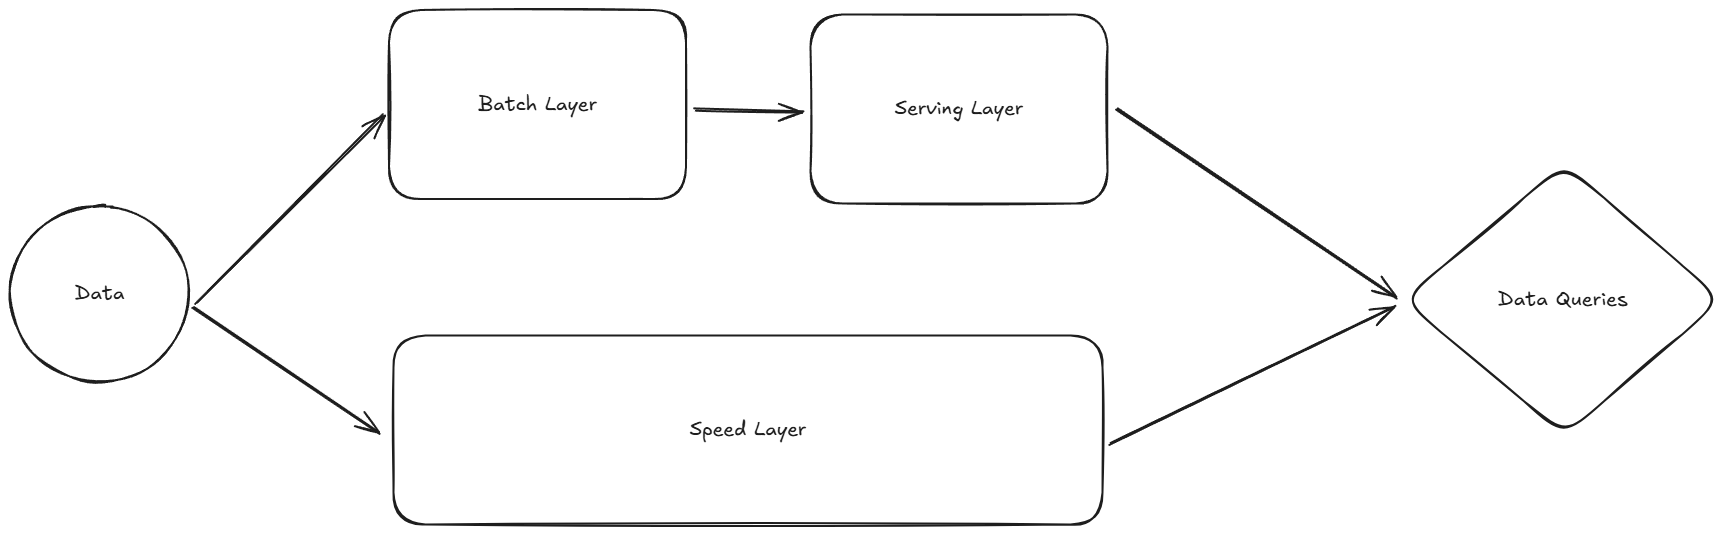
\includegraphics[width=0.8\textwidth]{teorico/arquitecturas/lambda.png}
\caption{Diagrama de la Arquitectura Lambda}
\label{fig:arquitectura_lambda}
\end{figure}
\clearpage
\newpage

\subsection{Capacidades}
\begin{itemize}
\item \textbf{Procesamiento de datos a gran escala}: Maneja eficientemente volúmenes masivos de datos.
\item \textbf{Baja latencia}: Proporciona resultados en tiempo real para consultas.
\item \textbf{Tolerancia a fallos}: Mantiene la integridad de los datos incluso en caso de fallos del sistema.
\item \textbf{Escalabilidad}: Se adapta fácilmente al crecimiento del volumen de datos.
\item \textbf{Flexibilidad}: Permite el procesamiento tanto batch como en tiempo real.
\item \textbf{Consistencia eventual}: Garantiza que los datos eventualmente reflejarán todos los cambios.
\item \textbf{Reprocesamiento}: En caso de necesitar reprocesar los datos, este proceso es trivial, pues se tiene almacenado el histórico completo.
\end{itemize}

\subsection{Desafíos}
\begin{itemize}
\item \textbf{Complejidad}: La implementación y mantenimiento pueden ser complejos debido a la duplicación de lógica en las capas de lotes y velocidad.
\item \textbf{Latencia}: El procesamiento batch genera latencia debido al tiempo de la actualización de vistas.
\item \textbf{Costo}: Al utilizar recursos computacionales diferentes entre el procesamiento batch y en stream, esto puede requerir varios nodos computacionales, lo que incrementa los costos.
\end{itemize}
\newpage